
\section{Aufbau und Durchführung}
\label{sec:Durchführung}

\subsection{Aufbau}
Wie in Kapitel \ref{sec:Theorie} beschrieben, wird die Lebensdauer der Myonen bestimmt, indem die Zeit zwischen Eintreffen und Zerfall eines Myons in einem Szintillator gemessen wird.
Dies wird durch den in Abbildung \ref{fig:1} dargestellten Aufbau realisiert.
Die in dem Szintillator entstehenden Photonen beim Eintreffen so wie beim Zerfallen der Myonen, werden durch die beiden Photomultiplier (PM) detektiert.
Die Signale der PM werden durch Verzögerungsleitungen, welche vorangegangene Verzögerungen der einzelnen PM ausgleichen, an Diskriminatoren angeschlossen.
Die Diskriminatoren unterdrücken alle Signale unterhalb eines bestimmten Schwellspannung U$_0$, wodurch thermische Anregungen der PM herausgefiltert werden.
Höher energetischer Untergrund wird durch die nachgeschaltete Koinzidenzschaltung herausgefiltert.
Diese gibt ein Signale nur weiter, wenn beide eingehende Signale innerhalb eines Zeitraumes $t_k$ eintreffen.
Durch die Kombination der beiden Filter, wird der größte Teil des unkorrelierten Untergrundes herausgefiltert.

\begin{figure}
    \centering
    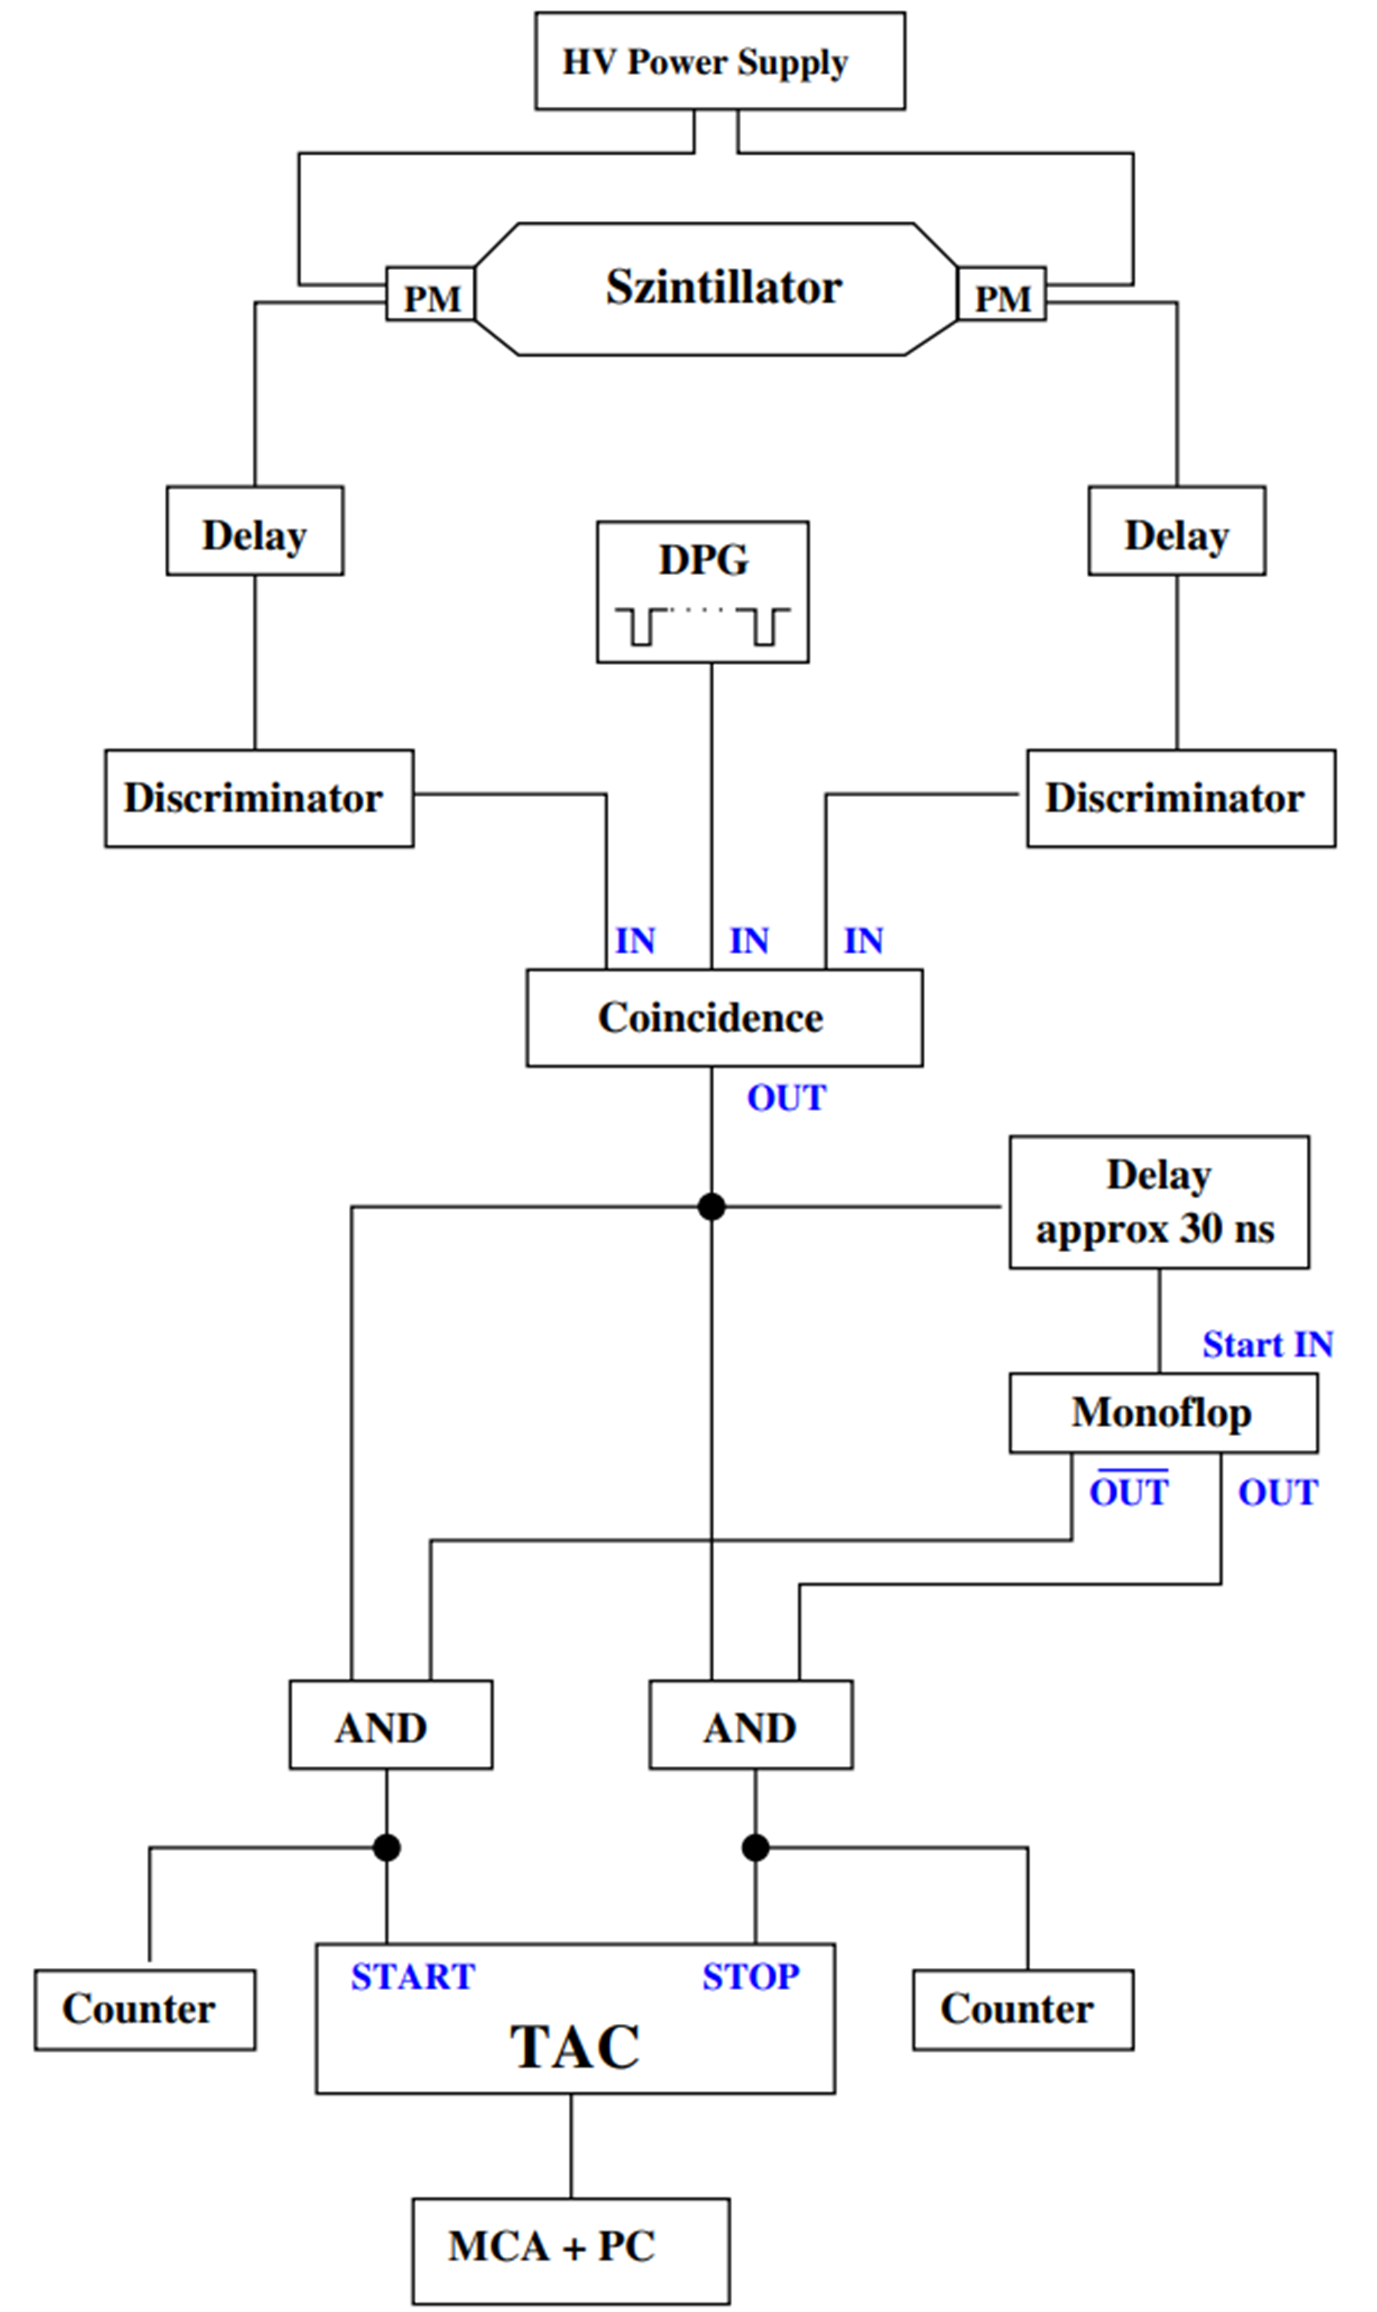
\includegraphics[width= 0.7\textwidth]{plots/V01_Aufbau.png}
    \caption{Skizze der Schaltung \cite{V01}.}
    \label{fig:1}
\end{figure}
Die gefilterten Signale werden nun in den Schaltungsteil weiter geleitet, der die Signale zählt, so wie die Lebensdauer misst, falls das Myon zerfällt.
Dafür wird das Signal in 3 Teile aufgeteilt.
Zwei Signale werden an je ein AND-Gatter angeschlossen. 
Das Dritte wird nach einer Verzögerung von $\SI{30}{\nano\second}$ an einen Monoflop angeschlossen.
Nachdem der Monoflop durch ein HIGH-Signal getriggert wurde, gibt er für die Zeit T$_S$, ein HIGH-Signal aus.
Dabei entspricht T$_S$ der Suchzeit, in der ein zweites eintreffendes Signal als Zerfall des vorher eingetroffenen Myons interpretiert wird.
Der Monoflop ist invertiert an das erste AND-Gatter und normal an das zweite AND-Gatter angeschlossen.
Ist die Schaltung im Ruhezustand, also der Monoflop nicht getriggert und es trifft ein Signal ein, so liegen am ersten AND-Gatter ein HIGH-Signale an.
Dieses wird weiter an den Impulszähler gegeben und startet den Zeit-Amplituden-Converter (TAC).
Am zweiten AND-Gatter liegen zur selben Zeit ein HIGH- und ein LOW-Signal an, daher wird kein Signal weiter geleitet.

Trifft nun innerhalb der Suchzeit T$_S$ ein weiteres Signal ein, so liegen durch den Aktivierten Monoflip ein HIGH- und ein LOW-Signal a, ersten AND-Gatter an, es wird kein Signal weiter geleitet.
Am zweiten AND-Gatter hingegen liegen jetzt zwei HIGH-Signale an, das Signal wird weiter geleitet.
Durch das Signal wird ein weiterer Impulszähler aktiviert, so wie der TAC gestoppt.
Der Zeit-Amplituden-Converter gibt nun eine Spannung weiter, die proportional zu der Zeit zwischen den beiden eingegangenen Signalen ist.
Diese Spannung wird an einen Multi-Channel-Analyser (MCA) geleitet, welcher durch einen PC ausgewertet wird.

\subsection{Durchführung}
Zunächst wird die Schaltung wie in Abbildung \ref{fig:1} aufgebaut und die einzelnen Komponenten eingestellt.
Als erstes werden die Dikriminatorschwellen so eingestellt, dass beide Diskriminatorendie gleiche Impulsrate von etwa 30 pro Sekunde haben.
Danach wird die Pulsrate der Koinzidenzschaltung in Abhängigkeit der Verzögerung durch die Verzögerungsleitungen gemessen.
Dies wird für die Pulsdauern $\Delta t = \SI{20}{\nano\second}$ und $\Delta t = \SI{10}{\nano\second}$, welche an den Diskriminatoren eingestellt werden können, durchgeführt.
Für den restlichen Versuch wird eine Pulsdauer von $\Delta t = \SI{10}{\nano\second}$ gewählt.
Anschließend werden die Verzögerungsleitungen so eingestellt, dass eine möglichst hohe Impulsrate von der Koinzidenzschaltung ausgegeben wird.
Zudem wird an dem Monoflop eine Suchzeit von $T_S = \SI{12}{\nano\second}$ eingestellt.
%Nun wird der TAC so eingestellt, dass möglichst viele Kanäle des MAC genutzt werden.
Nun werden der Tac und der MCA kalibriert, damit aus der Spannungshöhe bzw. dem Channel die Lebensdauer der Myonen bestimmt werden kann.
Dafür wird der Doppelimpulsgenerator an die Koinzidenzschaltung angeschlossen und für verschiedene Impulsabstände der entsprechende Channel notiert.
Am Ende wird die Messung der Lebensdauer der kosmischen Myonen gestartet.
Diese geht etwa drei Tage lang, während der die Start-, so wie Stopp-Signale gezählt und die Lebensdauern der Myonen am Computer erfasst werden.